% !TEX root =  ../main.tex
\section{CumulatedCapacity}

\subsection{Definition}

\subsubsection{Signature} \cstr{cumulatedCapacity(s:set<server>, r:string, nb:number)}

\begin{itemize}
\item \cstr{s}: a non-empty set of servers for a meaningful constraint. Servers not in the \st{Online} state are ignored.
\item \cstr{r} : a resource identifier such as \cstr{vm}, \cstr{mem}, \cstr{ucpu}, \cstr{pcpu} or \cstr{nodes} to identify the number of virtual machines, the physical memory, the computational capacity, the physical CPUs, respectively.
\item \cstr{nb}: a positive amount of resources. 
\end{itemize}

The \cstr{cumulatedCapacity} constraint restricts to a maximum of \cstr{nb}, the total amount
of a specific resource of type \cstr{r} that can be used on the online servers in \cstr{s} to run VMs.


\classification{cumulatedCapacity}{datacenter administrator}{VM placement,Resource allocation}{VM-to-server placement,Resource management}


\subsubsection{Usage}

The \cstr{cumulatedCapacity} constraint enables first the datacenter administrator to control 
the shared resources of
a platform. As an example, each VM has at least one IP address to be accessible from the network.
In practice, a datacenter has a finite pool of addresses to share among all the VMs.
Such a datacenter has then a global hosting capacity limited by the size of the address pool.
In this setting, one \cstr{cumulatedCapacity} constraint may be used to limit the hosting capacity
of VMs according to the size of the address pool.

The \cstr{cumulatedCapacity} constraint may also be used to control license restrictions.
As an example, on a datacenter running vSphere, the hosting capacity is limited by the cumulated amount of
memory allotted to the running VMs.~\cite{vsphere-license} In this setting, one \cstr{cumulatedCapacity}
constraint may be use by the datacenter administrator to guarantee the overall consumption of memory used
on the servers running VMWare is necessarily lesser to the maximum allowed by the acquired licenses.


\subsubsection{Example}

Figure~\ref{fig: cumulatedCapacity} depicts a sample reconfiguration between a source and a destination configuration where each server provides 8 unit of CPU and 7 unit of memory resources to VMs. Each VM is associated to a gray rectangle that denotes its resource usage. In this setting, the following \cstr{cumulatedCapacity} constraints were considered :

\begin{figure}[htb]
\centering
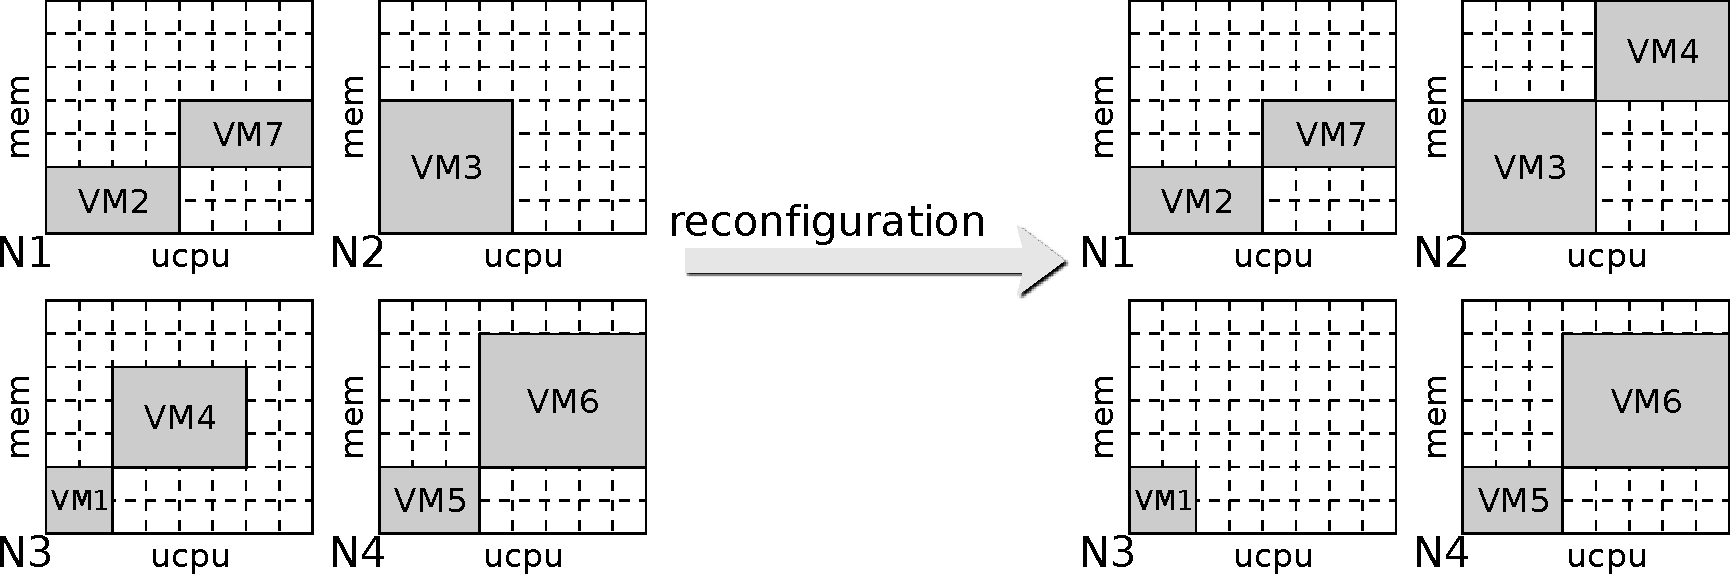
\includegraphics[width=\textwidth]{img/cumulatedCapacity}
\caption{A reconfiguration motivated by \cstr{cumulatedCapacity} constraints.}\label{fig: cumulatedCapacity}
\end{figure}


\begin{itemize}
\item \cstr{cumulatedCapacity(\{N1, N3\},7,"mem")}. This constraint was not satisfied in the source configuration as the cumulated memory usage on \cstr{N3} and \cstr{N1} was equals to 9.
This violation was fixed by relocating \cstr{VM4} to \cstr{N2}.

\item \cstr{cumulatedCapacity(\{N3, N4\},3,"vm")}. This constraint was not satisfied in the source configuration as there was
4 VMs running on the two nodes while the constraint restricts this number to 3 at maximum. This violation was fixed with the relocation of \cstr{VM4} to \cstr{N2}.

\item \cstr{cumulatedCapacity(\{N2, N4\},16,"ucpu")}. This constraint was satisfied in the source configuration as the cumulated UCPU usage of \cstr{N2} and \cstr{N4} was equals to 12. The constraint is still
satisfied in the destination configuration as the cumulated UCPU usage equals 16.
\end{itemize}


\fullVersion{
\subsection{Model}

This constraint is modeled by restricting the occurrences of d-slices hosted on the given servers.

\begin{equation*}
\begin{split}
\forall N \subseteq \mathcal{N},\ cumulatedCapacity(N, nb) \triangleq&\\
 & \forall v_i \in \mathcal{V},\ \sum_{d_i |�d_i^{host} \in n |�n \in {N}} d_i \leq nb
\end{split}
\end{equation*}

\subsection{Violation Detection}

The detection of the violating elements in \cstr{globalHostingCapacity} consists in counting VMs
that are hosted on the given server. When the amount of VMs is greater than the maximum
allowed, then the difference indicates the minimum number of VMs that are misplaced.
Such a detection is however not capable to indicate the VMs that are actually misplaced.


\subsection{Availability}

\subsubsection{In {\btrp}}

The constraint is available under the name \texttt{capacity} since version 2.1. The constraint is
modeled using one \emph{among}~\cite{among} constraint that directly counts the VMs assigned
to any server in the designated group of servers.

\begin{equation*}
\begin{split}
\forall N \subseteq \mathcal{N},\ globalHostingCapacity(N) \triangleq&\\
 & among(nb, \{ d_i^{host} | n_i \in N\}),
\end{split}
\end{equation*}
}
\subsection{See also}

\subsubsection{Related Constraints}
\begin{itemize}
\item \cstrref{singleCapacity}: A constraint to restrict the resource capacity on each server. A \cstr{cumulatedCapacity} constraint is then equivalent to a \cstr{single\-Capacity} constraint when the set of servers in \cstr{cumulatedCapacity} is a singleton.
\end{itemize}

\printListOfInheritance{cumulatedCapacity}